 Dans ce chapitre, nous attaquons le cœur de l'étude numérique dont l'objectif est de répondre à la question : quel est l'impact de la correction dépendant de l'anisotropie de pression sur le taux de cascade ? Les résultats montrés ici sont récents, préliminaires et leur interprétation est encore en cours de discussion.
 
 \section{Le modèle CGL simulé} \label{sec-331}
 
 Dans un premier lot de simulations, les ions sont décrits avec la fermeture \cacro{CGL} et les électrons avec une fermeture isotherme qui correspond à notre fermeture isotherme-isentrope. La contribution des flux de chaleur est supposée nulle. La pression électronique est définie telle que $p_e = \rho$. Le modèle général \sacro{CGLHPe} simulé dans le code versatile est donné dans la section \ref{sec-233}. Regardons à quoi il ressemble si l'on y injecte les fermetures et que l'on y applique la normalisation indiquée dans la section \ref{sec-311} et utilisée dans l'implémentation des équations. Les équations de ce modèle sont ainsi :
 \begin{eqnarray}
 \label{eq:mcgl_r} \partial_t \rho + \nabla \cdot \left(\rho \boldsymbol{v}\right) &=& 0,\\
 \label{eq:mcgl_v} \partial_t  \boldsymbol{v} + \boldsymbol{v} \cdot \nabla  \boldsymbol{v} - \frac{1}{\rho} \boldsymbol{j} \times \boldsymbol{B} + \frac{1}{\rho} \nabla \cdot \overline{\boldsymbol{P}}  &=& 0,  \\
 \label{eq:mcgl_b} \partial_t \boldsymbol{B} - \nabla \times \left( \boldsymbol{v} \times \boldsymbol{B} \right) +  d_i  \nabla \times \left( \frac{1}{\rho} \boldsymbol{j}\times \boldsymbol{B} \right) &=& 0 , \\
 \label{eq:mcgl_pperp} \partial_t  p_{\perp i }  +  \nabla \cdot \left(p_{\perp i } \boldsymbol{v} \right) +  p_{\perp i }\nabla \cdot\boldsymbol{v} -  p_{\perp i } \boldsymbol{b}\boldsymbol{b} : \nabla \boldsymbol{v}  &=& 0  ,\\
 \label{eq:mcgl_ppar} \partial_t  p_{\parallel i }  +  \nabla \cdot \left(p_{\parallel i } \boldsymbol{v} \right) +  2 p_{\parallel i }  \boldsymbol{b}\boldsymbol{b} : \nabla \boldsymbol{v}  &=& 0  ,
 \end{eqnarray}
 en notant $\overline{\boldsymbol{P}} =  \frac{\beta_0}{2} \left(\overline{\boldsymbol{P_i}} + \rho \overline{\boldsymbol{I}} \right)$ avec $\overline{\boldsymbol{P_i}} = p_{\perp i } \overline{\boldsymbol{I}} + \left(p_{\parallel i } - p_{\perp i }\right) \boldsymbol{b} \boldsymbol{b}$ le tenseur gyrotrope de pression ionique, $\boldsymbol{b} = \frac{\boldsymbol{B}}{|\boldsymbol{B}|}$ la direction du champ magnétique et $\frac{\beta_0}{2} $ une constante provenant de la normalisation des équations.
 
 L'hypothèse isotherme vient annuler la contribution $\nabla P_e$ présente dans l'équation d'induction \eqref{eq:model_simu_b} puisque : 
 \begin{equation*}
      \nabla \times \left( \frac{1}{\rho} \nabla \left(  p_e\right) \right) =  \nabla \times \left( \frac{1}{\rho} \nabla  \rho \right) = \nabla \times  \nabla \left( \ln \rho \right) = 0.
 \end{equation*}
 On s'attend donc à ce que la contribution de $\nabla P_e$ permettant de compenser l'effet de ce terme dans l'équation d'énergie totale s'annule aussi. L'énergie interne étant $\rho u = \frac{\beta_0}{2} \left(p_{\perp i } + \frac{1}{2}p_{\parallel i} + \rho \ln \rho \right) $, son équation peut en effet s'écrire :
 \begin{eqnarray}
 \label{eq:mcgl_ui} \partial_t \left(\rho u\right) + \nabla \cdot \left(\rho u \boldsymbol{v}\right) +  \overline{\boldsymbol{P}}: \nabla \boldsymbol{v} &=& 0.
 \end{eqnarray}
 
 On reconnaît dans ces équations le modèle ayant donné la loi exacte \eqref{eq:turb_cpg_elk} ainsi que le terme de \cacro{Hall} dans l'équation \eqref{eq:mcgl_b} qui indique qu'il faut prendre en compte la correction \cacro{Hall} donnée par \eqref{eq:corr_hall}. Le taux de transfert non linéaire $\varepsilon_{NL}$ obtenu, qui est aussi valable en dehors de la zone inertielle, sera noté $\varepsilon_{cgl}$. On le comparera à $\varepsilon_{iso}$ calculé avec la partie isotrope du tenseur de pression\footnote{Le comportement de $\varepsilon_{iso}$ est connu, il a été étudié par \cite{andres_energy_2018} dans le cas isotherme. Comme nous utilisons une nouvelle formulation de la loi exacte, une vérification des prédictions est détaillée dans l'Annexe \ref{an:compa_predict}.}. On s'attend, pour ces quantités, à observer une zone inertielle élargie de la zone \cacro{MHD} à la zone \cacro{Hall}. 
 La différence $\varepsilon_{\overline{\boldsymbol{\Pi}}}=\varepsilon_{cgl}-\varepsilon_{iso}$ correspond à la contribution de l'anisotropie de pression donnée par l'équation \eqref{eq:turb_cpgyr_an}. Elle sera décomposée en quatre termes : 
 \begin{itemize}
     \item un terme flux : $\nabla_{\boldsymbol{\ell}} \cdot \boldsymbol{\mathcal{F}_A} = \frac{1}{4} \nabla_{\boldsymbol{\ell}} \cdot \left< \delta \rho \delta \left(\frac{\overline{\boldsymbol{\Pi}}}{\rho}\right) \cdot \delta \boldsymbol{v} \right> $,
     \item le terme source survivant dans la limite incompressible : 
     \begin{equation*}
         \mathcal{S}_{A1} = \frac{1}{2}\left<  \delta \left(\frac{\overline{\boldsymbol{\Pi}}}{\rho}\right) : \left(\rho\nabla' \boldsymbol{v'} -  \rho'\nabla  \boldsymbol{v}\right)\right>,
     \end{equation*}
     \item le terme source compressible dépendant explicitement des fluctuations de pression : 
     \begin{equation*}
         \mathcal{S}_{A2} =  \frac{1}{4}  \left<\delta \left(\frac{\overline{\boldsymbol{\Pi}}}{\rho}\right) : \left(\rho \boldsymbol{v} \frac{\nabla' \rho'}{\rho'} -\rho'\boldsymbol{v'}  \frac{\nabla \rho}{\rho} \right)  \right>,
     \end{equation*}
     \item le terme source dépendant explicitement des fluctuations de densité : 
     \begin{equation*}
         \mathcal{S}_{A3} = - \frac{1}{4}\left< \delta \rho \left(  \boldsymbol{v} \cdot   \left(\frac{\overline{\boldsymbol{\Pi}}}{\rho}\right) \cdot  \frac{\nabla' \rho'}{\rho'} - \boldsymbol{v'} \cdot \left(\frac{\overline{\boldsymbol{\Pi'}}}{\rho'}\right) \cdot  \frac{\nabla \rho}{\rho}\right) \right>,
     \end{equation*}
 \end{itemize}
 avec $\overline{\boldsymbol{\Pi}} =  \frac{\beta_0}{2} \left(p_{\parallel i } - p_{\perp i }\right)\left( \boldsymbol{b} \boldsymbol{b} - \frac{1}{3}  \overline{\boldsymbol{I}} \right)$. Cette contribution anisotrope est entièrement portée par les ions.
 
 \section{Étude de la loi CGL-MHD-Hall-\ensuremath{\nabla P_e} dans les simulations CGL1, CGL2, CGL3}
 \label{sec-332} 
 
 Tout d'abord, nous avons entrepris l'analyse des simulations CGL1, CGL2 et CGL3.
 Ce sont les simulations \sacro{CGLHPe} analysées dans l'article de \cite{ferrand_fluid_2021}, leurs paramètres sont résumés dans la \tabref{tab:setups} et la \tabref{tab:setups_hd}. Ces trois simulations sont initialisées telles que $a_{pi} = 1$. 
 
 \subsection{Loi globale et contribution de l'anisotropie de pression}
 La \figref{fig:trip_CGL1-2} (CGL1 et CGL2) et la \figref{fig:trip_CGL3} (CGL3) contiennent des triptyques associés à chaque simulation et permettant de comparer les taux de cascade $\varepsilon_{iso} $ et  $\varepsilon_{cgl}$. La différence des deux $\varepsilon_{\overline{\boldsymbol{\Pi}}} $ est représentée en \sacro{2D} en fonction de $\ell_{\perp}$ et $\ell_{\parallel}$, et est projetée dans les représentations \cacro{1D} sous la forme de courbe verte. Sur les représentations \cacro{1D}, sont ajoutés $\varepsilon_{cgl}$ en bleu, $\varepsilon_{iso}$ en orange et le niveau d'incertitude $\zeta$ en gris qui reste assez éloigné des autres quantités.
 
 \begin{figure}[!ht]
  \centering
  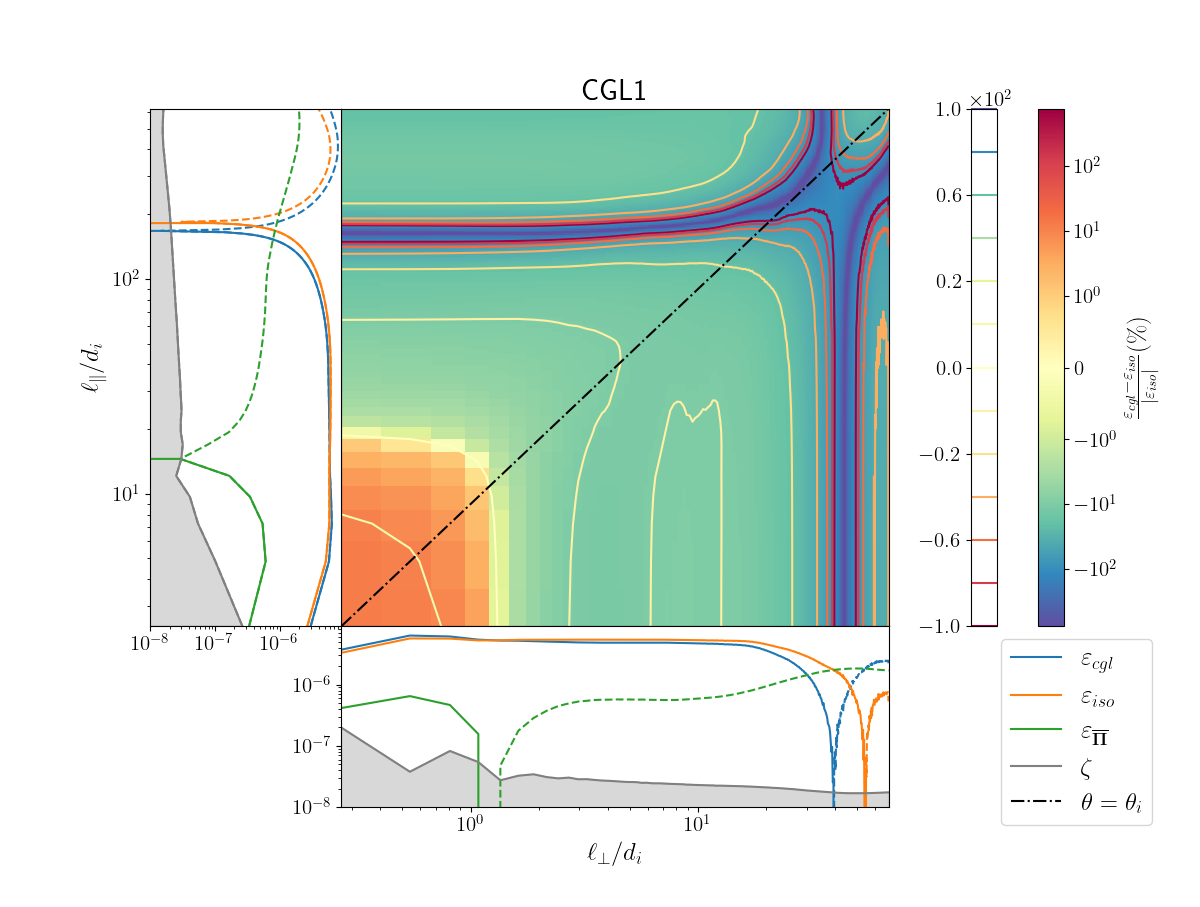
\includegraphics[width=0.95\linewidth,trim=1cm 0cm 0cm 2cm, clip=true]{./Mainmatter/Part_3/images_ch3/CGL1_panel_isocgl_percent}
 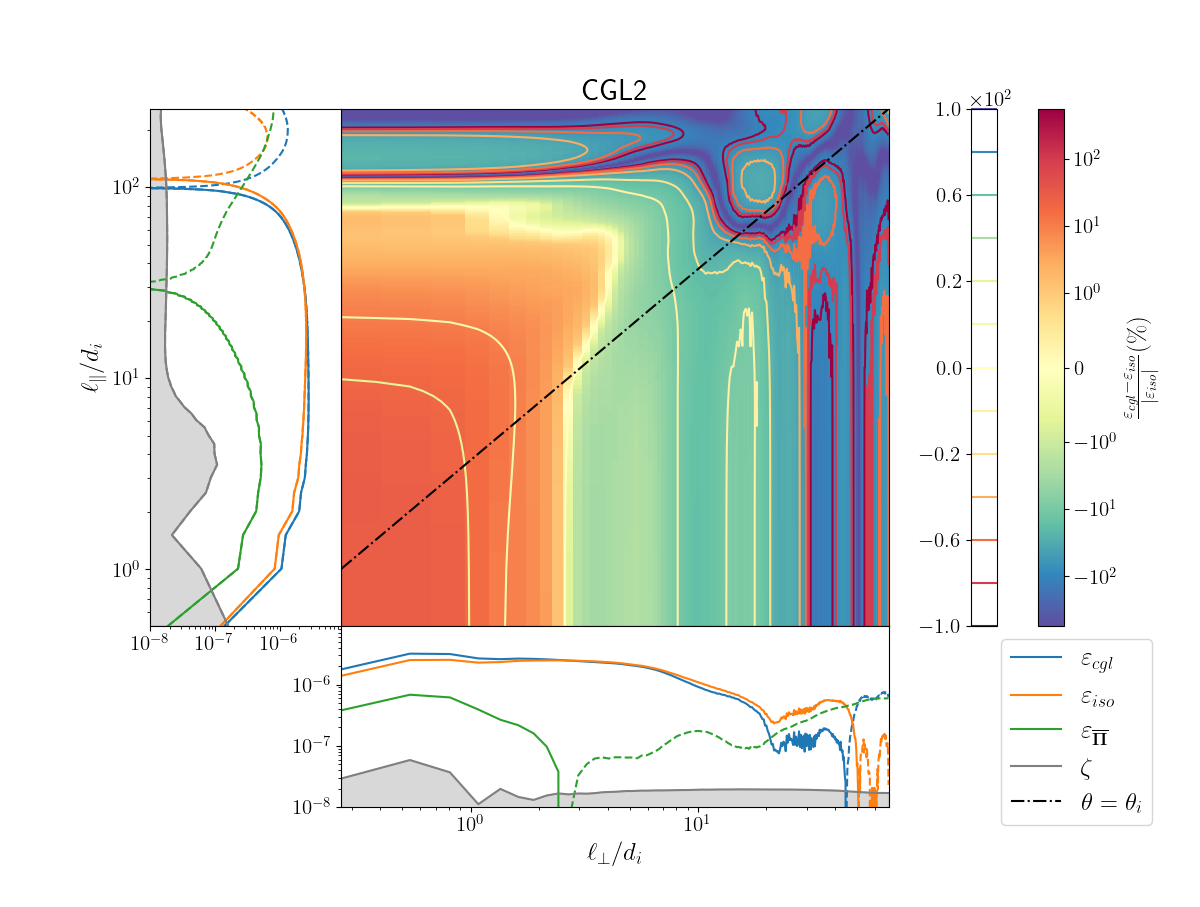
\includegraphics[width=0.95\linewidth,trim=1cm 0cm 0cm 2cm, clip=true]{./Mainmatter/Part_3/images_ch3/CGL2_panel_isocgl_percent}
 \cprotect\caption{Simu : CGL1 et CGL2. Représentation \cacro{2D} en fonction de \ensuremath{\ell_{\perp}} et \ensuremath{\ell_{\parallel}} de \ensuremath{\varepsilon_{cgl}-\varepsilon_{iso}} par rapport à \ensuremath{|\varepsilon_{iso}|} en \ensuremath{\%}, entourée des représentations \cacro{1D} en fonction de \ensuremath{\ell_{\perp}} (bas) et \ensuremath{\ell_{\parallel}} (gauche) de \ensuremath{\varepsilon_{iso}} (orange), \ensuremath{\varepsilon_{cgl}} (bleu), \ensuremath{\varepsilon_{\overline{\boldsymbol{\Pi}}}} (vert) et \ensuremath{\zeta} (gris). }
 \label{fig:trip_CGL1-2}
 \end{figure}
 \begin{figure}[!ht]
  \centering
 % 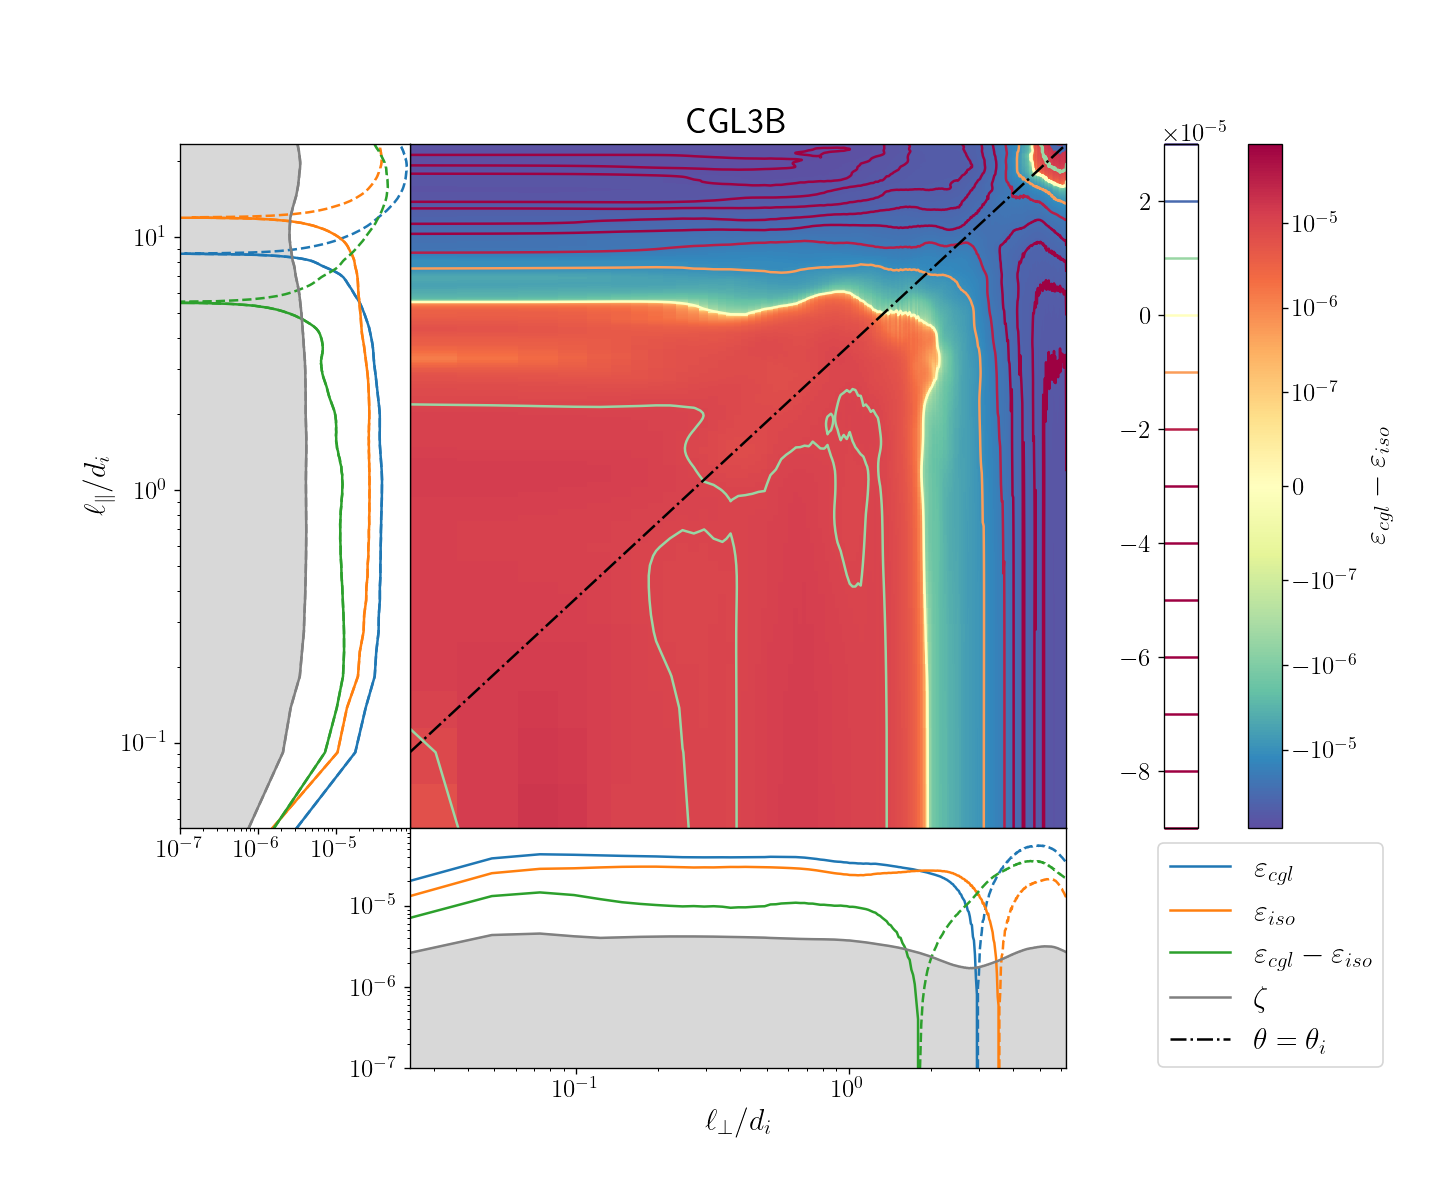
\includegraphics[width=0.95\linewidth,trim=0cm 2cm 0cm 3.5cm, clip=true]{./Part_3/images_ch3/CGL3B_panel_isocgl}
 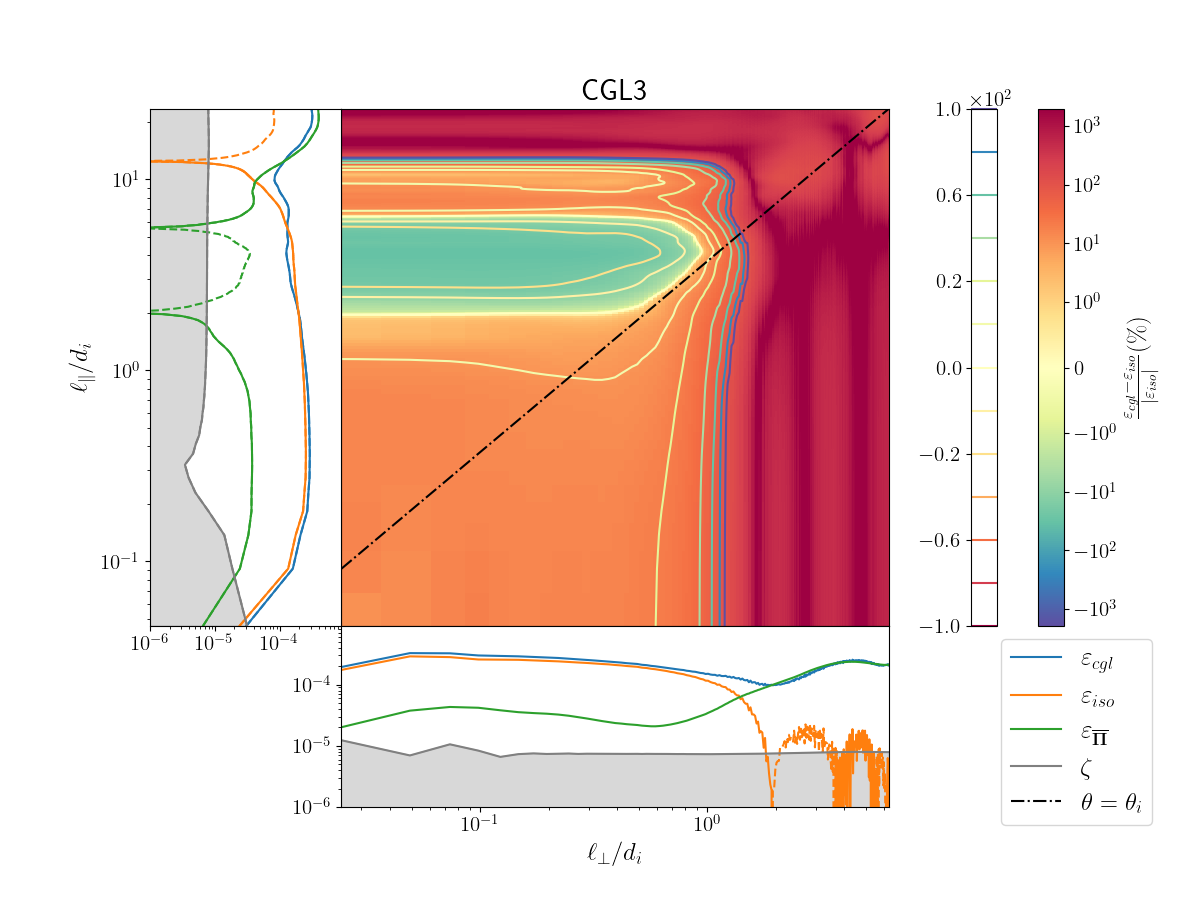
\includegraphics[width=0.95\linewidth,trim=1cm 1cm 0cm 2cm, clip=true]{./Mainmatter/Part_3/images_ch3/CGL3_panel_isocgl_percent}
 \cprotect\caption{Simu : CGL3. Représentation \cacro{2D} en fonction de \ensuremath{\ell_{\perp}} et \ensuremath{\ell_{\parallel}} de \ensuremath{\varepsilon_{cgl}-\varepsilon_{iso}} par rapport à \ensuremath{|\varepsilon_{iso}|} en \ensuremath{\%}, entourée des représentations \cacro{1D} en fonction de \ensuremath{\ell_{\perp}} (bas) et \ensuremath{\ell_{\parallel}} (gauche) de \ensuremath{\varepsilon_{iso}} (orange), \ensuremath{\varepsilon_{cgl}} (bleu),  \ensuremath{\varepsilon_{\overline{\boldsymbol{\Pi}}}} (vert) et \ensuremath{\zeta} (gris).}
 \label{fig:trip_CGL3}
 \end{figure}
 
 À partir de ces figures, on peut définir une zone inertielle où $\varepsilon_{cgl}$ sera quasi-constant pour chaque simulation. Pour CGL1, elle s'étend entre $\ell_{\perp} \in [\num{1};\num{20}]$ et $\ell_{\parallel} \in [\num{10};\num{60}]$, pour CGL2 entre $\ell_{\perp} \in [\num{1};\num{6}]$ et $\ell_{\parallel} \in [\num{2};\num{40}]$, et pour CGL3 entre $\ell_{\perp} \in [\num{0.1};\num{1}]$ et $\ell_{\parallel} \in [\num{0.2};\num{2}]$. Les variations que l'on pourra observer en dehors de ces domaines seront sous influence dissipative ou dans la zone de forçage. On remarque que la zone inertielle de CGL1 et CGL2 couvrent les échelles \cacro{MHD} et celle de CGL3, les échelles \cacro{Hall}. Dans ces zones, la contribution de $\varepsilon_{\overline{\boldsymbol{\Pi}}}$ au taux de cascade totale est en valeurs absolues d'environ $\SI{10}{\%}$ de $\varepsilon_{iso}$ pour CGL1 et CGL3, et entre $\SI{2}{\%}$ et $\SI{20}{\%}$ pour CGL2 (on prendra la valeur médiane : $\SI{10}{\%}$). Ce niveau reste donc constant. 
 
 Cependant, une différence de taille apparaît autour des grandes échelles de CGL3 (\figref{fig:trip_CGL3}) : $\varepsilon_{\overline{\boldsymbol{\Pi}}}$ augmente autour de $\num{10}$ fois la valeur de $\varepsilon_{iso}$. En pratique, on ne regarde pas ce qu'il se passe à ces échelles car elles sont impactées par l'injection d'énergie dans la cascade qui a tendance à faire fortement fluctuer les résultats provenant des lois calculées jusqu'à présents dans la littérature. Donc a priori, cette augmentation n'aurait pas un sens physique généralisable et serait plus spécifique à l'outil numérique. Pourtant, contrairement à l'impact du forçage observé dans la section \ref{sec-322}, il n'est pas oscillant et il provient spécifiquement de la contribution anisotrope. On s'est alors posé la question de son origine et de sa nature.
 
 Une autre différence est visible. Sur la représentation \sacro{2D} de CGL3 (\figref{fig:trip_CGL3}), la contribution anisotrope est positive quasiment partout à l'exception d'une \og bulle \fg{} accrochée à la direction parallèle. Tandis que pour CLG1 et CGL2 (\figref{fig:trip_CGL1-2}), un changement de signe de $\varepsilon_{\overline{\boldsymbol{\Pi}}}$ dans la zone inertielle \cacro{MHD} ($\ell > d_i$) semble indiquer une échelle caractéristique. Aux plus petites échelles, il est positif et puis devient négatif. L'emplacement de ce changement de signe est situé autour de $\ell^{s}_{\perp} \sim 2d_i$ dans la direction perpendiculaire. Dans la direction parallèle, le changement de signe a lieu en $\ell^{s}_{\parallel} \sim 20d_i$ pour CGL1, $\ell^{s}_{\parallel} \sim 80d_i$ pour CGL2. Trois éléments pourraient potentiellement expliquer ces observations. 
Tout d'abord, en présence d'un champ magnétique, le développement de la cascade est anisotrope comme on peut facilement le visualiser sur les cartes de \cite{manzini_local_2022}. Cela pourrait venir expliquer l'observation $\ell^{s}_{\perp}<\ell^{s}_{\parallel}$. Ensuite, l'angle d'injection $\theta_i$ étant inférieur à $\ang{45}$, l'énergie n'est pas injectée isotropiquement dans la simulation. Il diffère d'ailleurs entre CGL1 ($\ang{7}$) et CGL2-CGL3 ($\ang{15}$). Si le premier élément est validé, cela pourrait impliquer que l'angle d'injection pourrait venir contrer ou amplifier l'anisotropie de $\varepsilon_{\overline{\boldsymbol{\Pi}}}$. Enfin, entre CGL2 et CGL3, la gamme d'échelles diffère ainsi que le niveau énergétique ($E_{sup}$), plus important pour CGL3.

 Le comportement dans la direction parallèle semblant plus complexe que celui de la direction perpendiculaire, on s'est focalisé sur la compréhension de cette dernière.
 Puisque le changement de signe a lieu près de la zone \cacro{Hall}, on s'est demandé si le comportement de CGL2 et celui de CGL3 ne se complétaient pas : l'augmentation présente dans CGL3 serait-elle le début d'une bosse qui ensuite se répercuterait aux échelles  \cacro{MHD} où sa diminution irait jusqu'à engendrer un croisement de $\varepsilon_{cgl}$ et $\varepsilon_{iso}$ et un changement de signe de $\varepsilon_{\overline{\boldsymbol{\Pi}}}$ ? Ce point est intéressant, car une telle bosse pourrait être la signature d'instabilités qui viendraient injecter de l'énergie aux échelles ioniques. Cette première question est mise en doute par le comportement de CGL1 et CGL2 : une augmentation similaire semble apparaître dans $\varepsilon_{\overline{\boldsymbol{\Pi}}}$  mais avec un signe opposé et une intensité moindre n'influant que très peu sur $\varepsilon_{cgl}$. Si c'est bien le même effet que pour CGL3, il serait alors accroché aux échelles de forçage. 
 Plus de questions que de réponses émergent donc de ces simulations, elles ont emmené l'analyse dans diverses directions nécessitant de nouvelles simulations : 
 \begin{itemize}
     \item le niveau de la zone inertielle changera-t-il si l'on initialise la simulation avec une pression anisotropique ($a_{piI} \neq 1$) ? 
     \item l'augmentation à grande échelle est-elle accrochée aux échelles de forçage ?
    \item le changement de signe de  $\varepsilon_{\overline{\boldsymbol{\Pi}}}$ est-il lié à la proximité de la frontière entre les zones \cacro{MHD} et \cacro{Hall} ?
     \item ces différences sont-elles des signatures de phénomène physique ? Sont-elles liées ?
 \end{itemize}
 Avant de se lancer dans de nouvelles simulations, d'autres élements peuvent être étudiés. Ils font l'objet des sections suivantes.  
 
 \subsection{Détail de la contribution de l'anisotropie de pression}
 
 \begin{figure}[!ht]
  \centering
  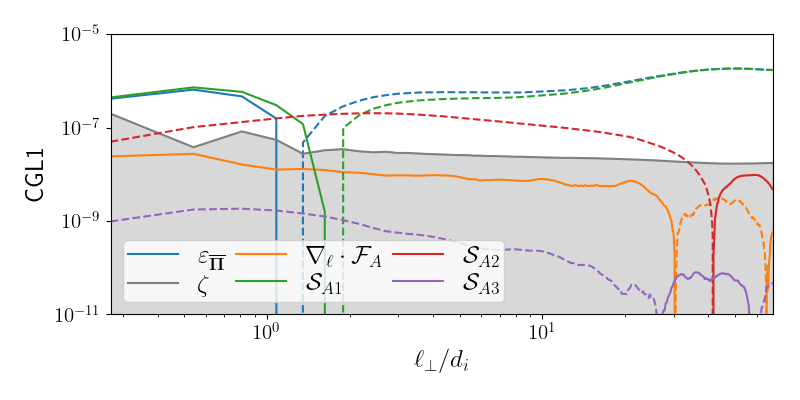
\includegraphics[width=0.9\linewidth,trim=0cm 0cm 0cm 0.5cm, clip=true]{./Mainmatter/Part_3/images_ch3/CGL1_compa_cgl}
 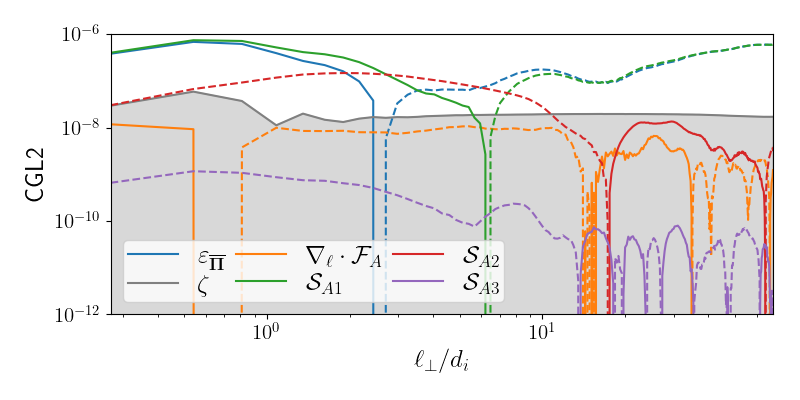
\includegraphics[width=0.9\linewidth,trim=0cm 0cm 0cm 0.5cm, clip=true]{./Mainmatter/Part_3/images_ch3/CGL2_compa_cgl}
  \includegraphics[width=0.9\linewidth,trim=0cm 0cm 0cm 0.5cm, clip=true]{./Mainmatter/Part_3/images_ch3/CGL3_compa_cgl}
 \cprotect\caption{Simu : CGL1 (haut), CGL2 (milieu) et  CGL3 (bas). Représentation \cacro{1D} en fonction de \ensuremath{\ell_{\perp}} du détail de \ensuremath{\varepsilon_{\overline{\boldsymbol{\Pi}}}} (bleu). Orange : \ensuremath{\nabla_{\boldsymbol{\ell}} \cdot \boldsymbol{\mathcal{F}_A}}. Vert : \ensuremath{\mathcal{S}_{A1}}. Rouge : \ensuremath{\mathcal{S}_{A2}}. Violet : \ensuremath{\mathcal{S}_{A3}}. Gris : niveau d'erreur \ensuremath{\zeta}. Les termes présents dans la zone grise délimitée par \ensuremath{\zeta} sont supposés négligeables. }
 \label{fig:detail_simu_CGL1-2}
 \end{figure}
 
 Sur la \figref{fig:detail_simu_CGL1-2}, est indiqué le détail de $\varepsilon_{\overline{\boldsymbol{\Pi}}}$ (bleu). On remarque que sont comportement est dominé par $\mathcal{S}_{A1}$ tandis que $\nabla_{\boldsymbol{\ell}} \cdot \boldsymbol{\mathcal{F}_A}$ et $\mathcal{S}_{A2}$ fluctuent autour de $\zeta$. Ils peuvent légèrement influencer $\varepsilon_{\overline{\boldsymbol{\Pi}}}$ lorsque $\mathcal{S}_{A1}$ s'affaiblit pour changer de signe, comme on peut le voir sur les résultats de CGL1 et CGL2. $\mathcal{S}_{A3}$ est, quant-à-lui, généralement négligeable. La contribution de l'anisotropie de pression et son comportement est donc principalement portée par le terme source qui survit dans la limite incompressible. Cela concorde avec la quasi-incompressibilité des simulations : l'écart-type de la densité est entre $\SI{2}{\%}$ (CGL1 et CGL2) et $\SI{8}{\%}$ (CGL3) de la moyenne. $\mathcal{S}_{A1}$ et $\varepsilon_{\overline{\boldsymbol{\Pi}}}$ doivent donc se comporter en accord avec la limite quasi-incompressible \eqref{eq:turb_cpinc_gyr1} obtenue dans le Chapitre \ref{ch-22} : 
 \begin{equation}
     \varepsilon_{\overline{\boldsymbol{\Pi}}} \simeq \mathcal{S}_{A1} \simeq \frac{\beta_0}{4}  \left< \delta \left(\left(p_{\parallel i } - p_{\perp i }\right)\left( \boldsymbol{b} \boldsymbol{b} - \frac{1}{3}  \overline{\boldsymbol{I}} \right) \right):\delta \left(\nabla \boldsymbol{v} \right)\right>
 \end{equation}
 Comprendre le comportement de ce terme est complexe puisqu'il dépend des fluctuations de la direction du champ magnétique $\boldsymbol{b}$ pondérées par l'anisotropie de la pression et distribuées sur les variations du gradient de la vitesse. $p_{\parallel i } - p_{\perp i }$ portant l'influence de l'anisotropie de pression de ce terme sur la loi exacte et pouvant s'écrire $1-a_{pi}$, on s'est intéressé au comportement statistique de $a_{pi}$. On remarque que seule la direction du champ magnétique influe sur ce terme et non son amplitude.
 
 Ces résultats sont retrouvés dans les simulations qui seront étudiées par la suite (voir Annexe \ref{an:Pi}).
 
 \subsection{Comportement statistique des pressions}
 
 La \tabref{tab:stat_CGL} résume la statistique (moyenne $\pm$ écart-type) des valeurs de la densité, de l'anisotropie de pression ionique $a_{pi} = \frac{p_{\perp i}}{p_{\parallel i}}$, et du paramètre $\beta_{\parallel} = \frac{p_{\parallel i}}{p_{m}}$ pour chaque simulation. Sur la figure \figref{fig:diag_simu_CGL}, est tracée la dispersion en fonction de $a_{pi}$ et $\beta_{\parallel}$, des simulations. Ces histogrammes \sacro{2D} prennent la forme de trois courbes de niveau formant des ovales concentriques. Le plus large contient tous les couples $\{\beta_{\parallel};a_{pi}\}$ existant dans la simulation, l'intermédiaire et le plus petit sont associés à des pourcentages du maximum de l'histogramme : $\SI{50}{\%}$ et $\SI{99}{\%}$. Sur cette figure, les critères des instabilités miroir et firehose ainsi que l'horizontale $a_{pi} =  1$ sont aussi affichés. Le critère firehose est le critère calculé dans le chapitre \ref{ch-21}, sa position sera affectée par l'effet \cacro{Hall}. Le critère miroir prend en compte la présence de la pression électronique isotherme $p_e = \rho$ et est paramétrisé par l'équation \eqref{eq:crit_miroir_elec}. Les simulations que l'on étudie ici sont données en 
 gris (CGL1), bleu (CGL2) et orange (CGL3) et correspondent aux première, deuxième et quatrième lignes du tableau. 
  \begin{table}[!ht]
 \begin{center}
 \begin{tabular}{ c|c|c|c } 
 Name & $\rho$ & $a_{pi}$  & $\beta_{\parallel}$\\
 \hline
 CGL1 & $\num{1}\pm \num{0.02}$ & $\num{1.1}\pm \num{0.1}$ & $\num{0.9}\pm \num{0.1}$ \\
 CGL2 & $\num{1}\pm \num{0.02}$ & $\num{1.1}\pm \num{0.1}$ & $\num{0.9}\pm \num{0.1}$   \\
 CGL3B & $\num{1}\pm \num{0.04}$ & $\num{1.3}\pm \num{0.3}$ & $\num{0.8}\pm \num{0.2}$   \\
 CGL3 & $\num{1}\pm \num{0.08}$ & $\num{2.2}\pm \num{0.5}$ & $\num{0.6}\pm \num{0.3}$  \\
 CGL5 & $\num{1}\pm \num{0.02}$ & $\num{2.1}\pm \num{0.1}$ & $\num{0.6}\pm \num{0.1}$  \\
 CGL6 & $\num{1}\pm \num{0.02}$ & $\num{3.97}\pm \num{0.5}$ & $\num{1.01}\pm \num{0.2}$  \\
 \end{tabular}
 \caption{Moyenne et écart-type de la densité, du taux d'anisotropie ionique $a_{pi} = \frac{p_{\perp i}}{p_{\parallel i}}$ et du paramètre $\beta_{\parallel} = \frac{p_{\parallel i}}{p_{m}}$ pour chaque simulation, à la date $t$. }\label{tab:stat_CGL}
 \end{center}
 \end{table}
 \begin{figure}[!ht]
  \centering
 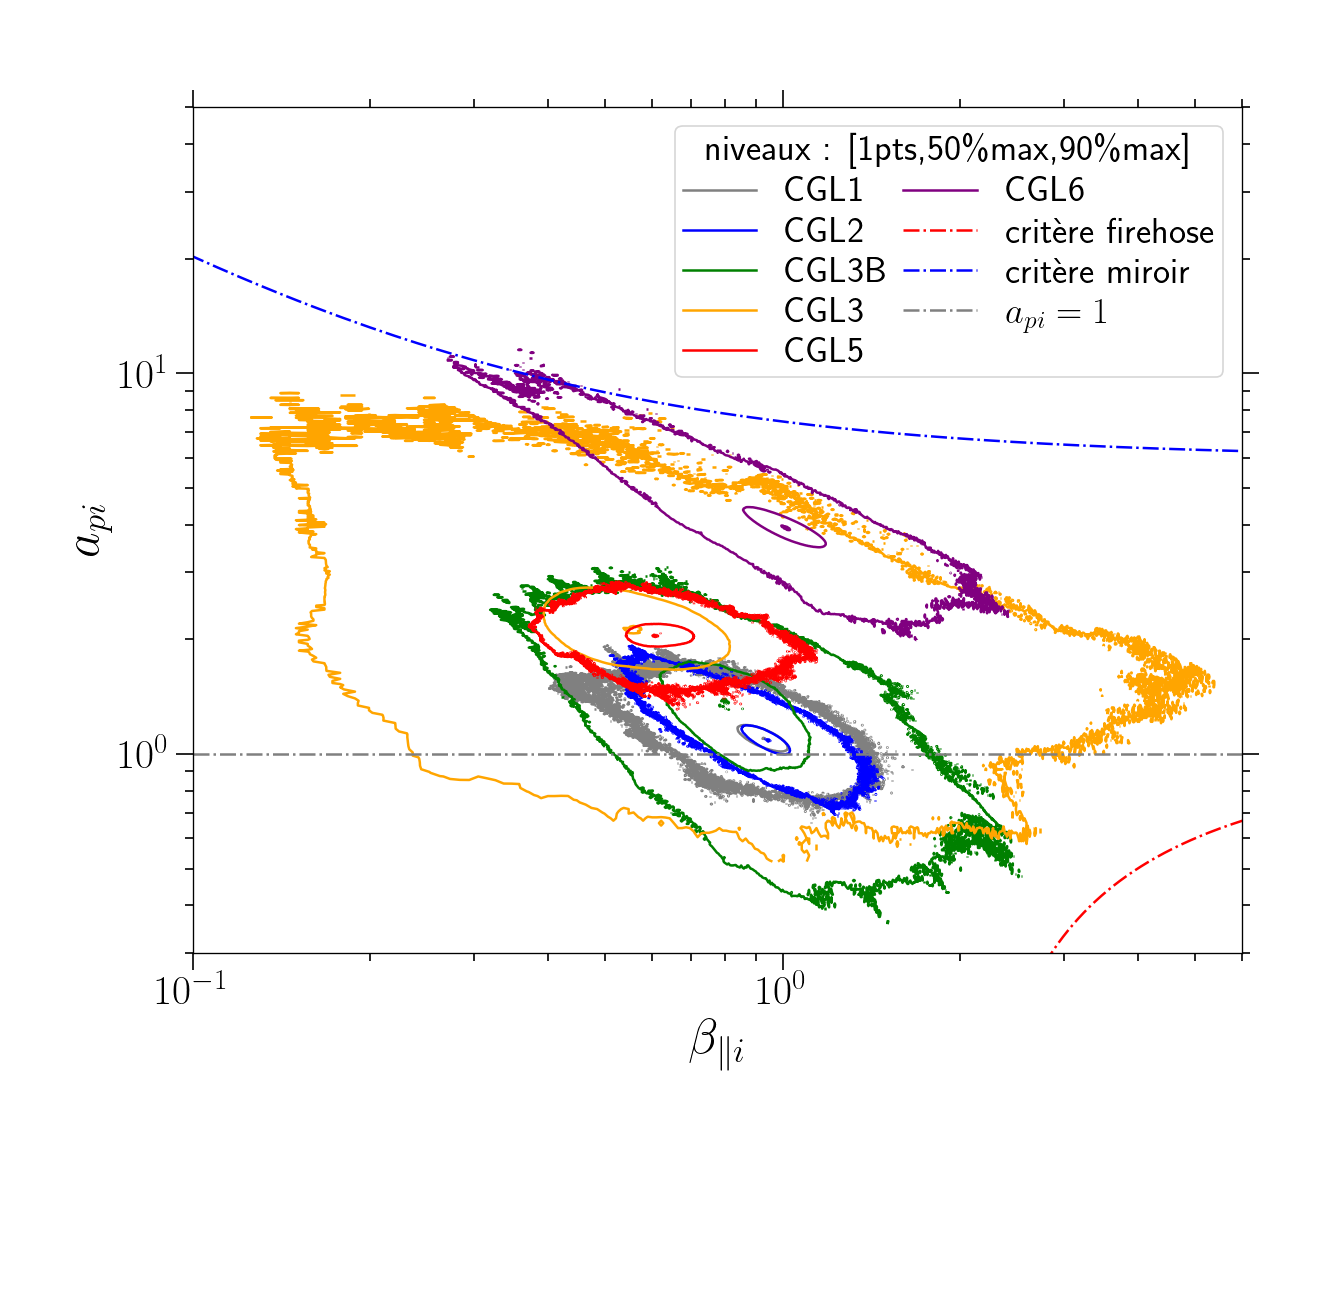
\includegraphics[width=0.8\linewidth,trim=1cm 7cm 2cm 1cm, clip=true]{./Mainmatter/Part_3/images_ch3/diag_apbeta}
 \cprotect\caption{Diagramme \ensuremath{a_{pi}-\beta_{\parallel}} contenant l'histogramme \sacro{2D} des simulations sous la forme de courbes de niveau centrées sur le couple moyen. Le critère miroir est paramétrisé par l'équation \eqref{eq:crit_miroir_elec} qui prend en compte les électrons isothermes. Le critère firehose est le critère \cacro{CGL} calculé dans le Chapitre \ref{ch-21}. }
 \label{fig:diag_simu_CGL}
 \end{figure} 
 
 On remarque que les trois simulations se sont écartées de leurs valeurs d'initialisation, $a_{piI} = 1$ et $\beta_{\parallel I} = 1$. $ \mathcal{S}_{A1}$ ne dépendant pas de $p_m$, on ne s'est pas attardé sur $\beta_{\parallel} = 1$.  Les distributions de CGL1 et de CGL2 sont quasiment identiques et très proches des valeurs initiales. CGL3 s'est quant-à-elle bien décalée et montre une moyenne $a_{pi0}\sim 2$, sa distribution est aussi beaucoup plus large avec quelques points proches du critère miroir. L'augmentation de la pression a lieu dès les premiers temps de la simulation puis reste stable. La raison d'un tel comportement est encore sujette à question : notre conjecture est qu'il est dû à l'énergie présente dans CGL3. Cette dernière est en effet forcée avec des ondes plus intenses et telle que l'énergie dans le système soit trois fois supérieure à celle dans CGL1 ou CGL2 (voir resp. $A_f$ et $E_{sup}$). Entre les points proches du critère miroir et l'augmentation de la moyenne et de l'écart-type de $a_{pi}$, beaucoup d'éléments pourraient être à l'origine de la différence de comportement de la contribution anisotrope. Ces résultats motivent d'autant plus l'obtention de nouvelles simulations. 
 
 \section{De nouvelles simulations}\label{sec-333}
 
 Trois nouvelles simulations ont été utilisées : CGL3B, CGL5 et CGL6. CGL5 et CGL6 ont été conçues et lancées pour répondre à certaines de nos questions. Comme indiqué dans le Chapitre \ref{ch-31}, obtenir des résultats de simulation valables pour une étude de turbulence prend du temps, c'est-à-dire plusieurs mois en comptant l'ajustement des paramètres d'hyperdissipation et, sachant qu'à chaque augmentation de la résolution, le temps de calcul était au moins multiplié par huit. Ainsi, d'une semaine de calcul pour faire converger le spectre associé à une résolution $258^2\times 512$, on passe à un ou deux mois pour $512^2 \times 1024$. Par conséquent, les résultats présentés ici sont récents et leur interprétation est encore en cours. 
 
 \subsection{Moins d'énergie que CGL3 : CGL3B}
 \begin{figure}[!ht]
  \centering
  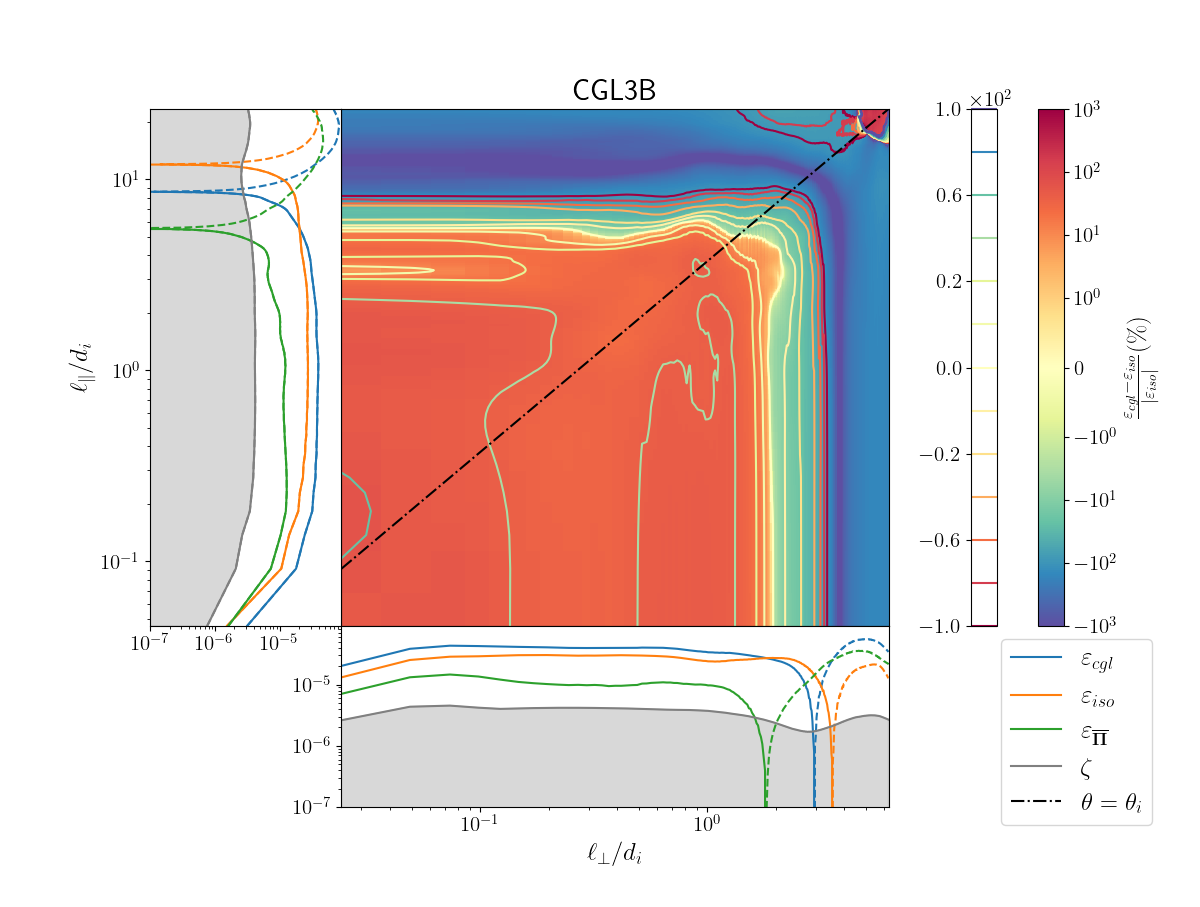
\includegraphics[width=0.95\linewidth,trim=1cm 1cm 0cm 2cm, clip=true]{./Mainmatter/Part_3/images_ch3/CGL3B_panel_isocgl_percent}
 %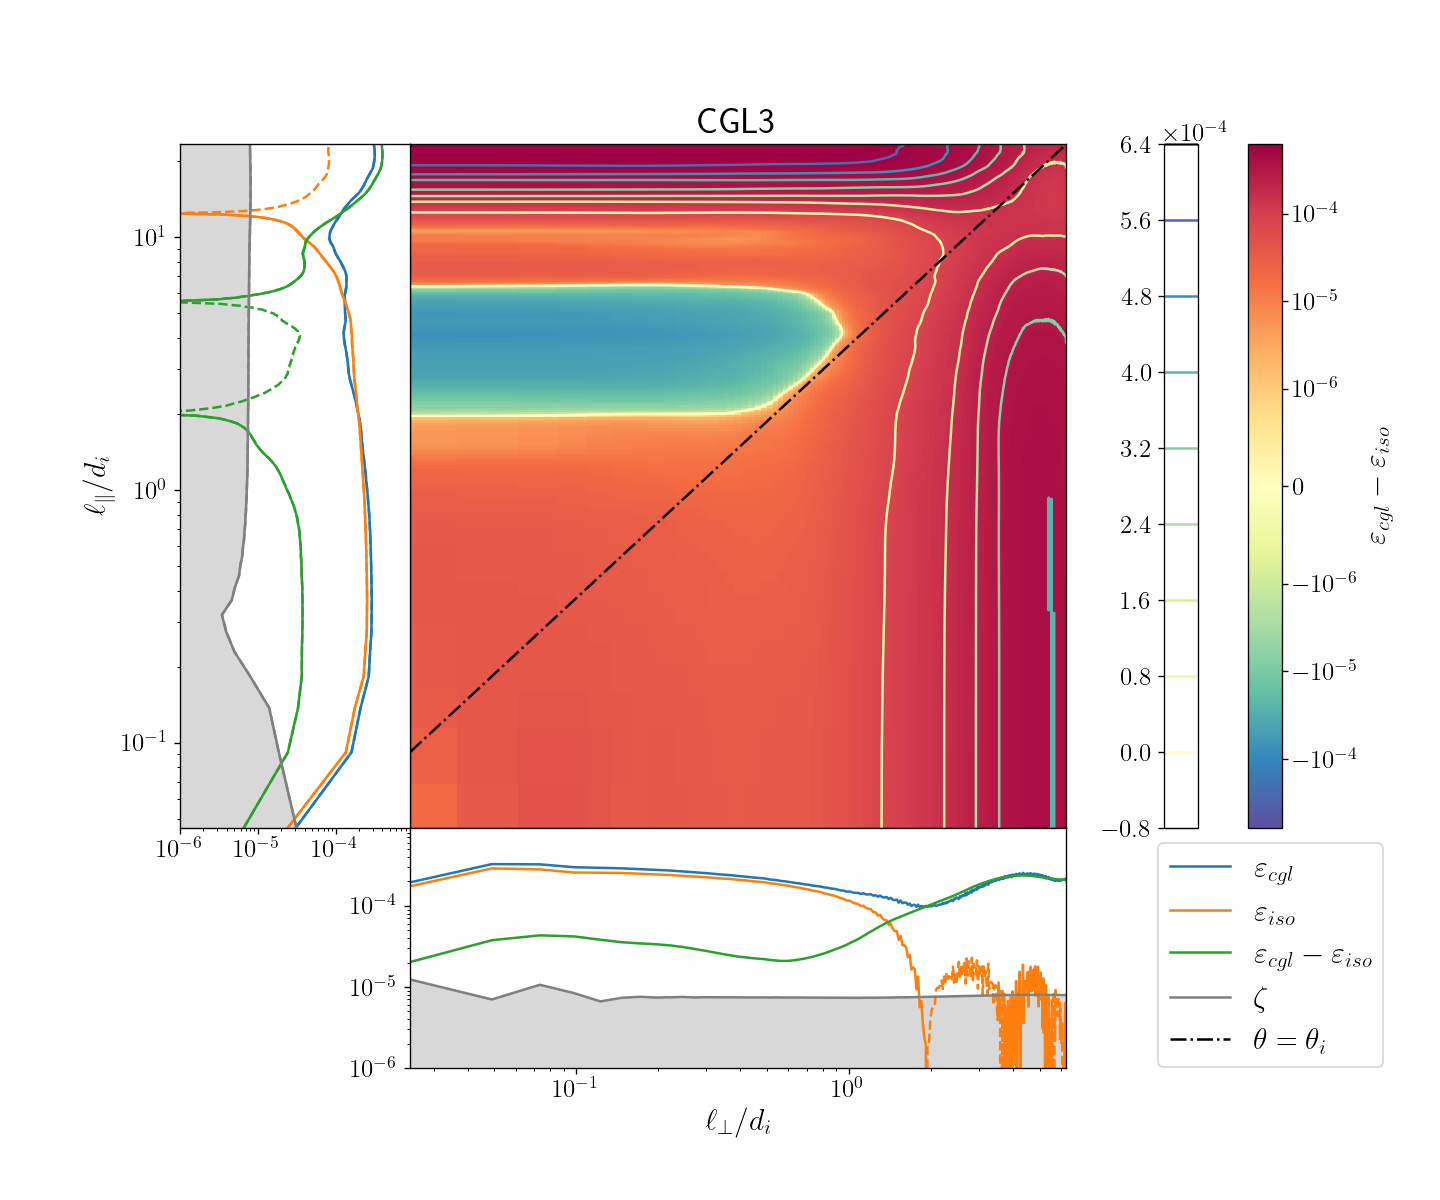
\includegraphics[width=0.95\linewidth,trim=0cm 2cm 0cm 3.5cm, clip=true]{./Part_3/images_ch3/CGL3_panel_isocgl}
 \cprotect\caption{Simu : CGL3B. Représentation \sacro{2D} en fonction de \ensuremath{\ell_{\perp}} et \ensuremath{\ell_{\parallel}} de \ensuremath{\varepsilon_{cgl}-\varepsilon_{iso}} par rapport à \ensuremath{|\varepsilon_{iso}|} en \ensuremath{\%}, entourée des représentations \cacro{1D} en fonction de \ensuremath{\ell_{\perp}} (bas) et \ensuremath{\ell_{\parallel}} (gauche) de \ensuremath{\varepsilon_{iso}} (orange), \ensuremath{\varepsilon_{cgl}} (bleu), \ensuremath{\varepsilon_{\overline{\boldsymbol{\Pi}}}} (vert) et \ensuremath{\zeta} (gris). }
 \label{fig:trip_CGL3B}
 \end{figure}
 Tout d'abord, CGL3B est une version moins énergétique de CGL3. La gamme d'échelle est donc la même, seul le forçage et par conséquent la dissipation sont affaiblis. Cette simulation est, elle aussi, initialisée telle que $a_{piI} = 1$. Sur le diagramme de la \figref{fig:diag_simu_CGL}, elle est indiquée en vert : sa moyenne, $a_{pi0} \sim 1.5$,  est entre celle de CGL2 et CGL3, et sa distribution inclue celle de CGL2 mais est moins étalée que celle de CGL3. On s'attend donc à voir les différences les plus importantes entre les résultats de l'étude des lois exactes de CGL2 et de CGL3 s'atténuer si $a_{pi}$ a de l'importance dans l'expression de la correction anisotrope.  Le triptyque fait l'objet de la \figref{fig:trip_CGL3B}. %Les contributions purement compressibles de $\varepsilon_{\overline{\boldsymbol{\Pi}}}$ étant ici aussi négligeable, on ne donnera pas son détail.
 
 À première vue, en regardant la représentation \sacro{2D}, on sait que l'on a un comportement similaire à CGL2. Le croisement entre $\varepsilon_{cgl}$ et $\varepsilon_{iso}$ dû au changement de signe de $\varepsilon_{\overline{\boldsymbol{\Pi}}}$ est toujours présent dans la zone \cacro{MHD}. Comme pour CGL3, cette zone est aussi la zone de forçage. Dans cette zone, on remarque une augmentation de la contribution venant dominer $\varepsilon_{iso}$. Si ces deux éléments ne sont pas des artefacts dus à l'oscillation du forçage, cela signifie que, contrairement à CGL3 et similairement à CGL1 et CGL2, le changement de signe a lieu avant l'augmentation, et cela tend à indiquer que l'augmentation présente dans CGL3 est intrinsèque à la zone de forçage.
 
 La zone inertielle est située entre $\ell_{\perp} \in [\num{0.1};\num{2}]$ et $\ell_{\parallel} \in [\num{0.2};\num{4}]$. Cette fois-ci, $\varepsilon_{\overline{\boldsymbol{\Pi}}}$ contribue à $\SI{30}{\%}$ de $\varepsilon_{iso}$. On a donc un facteur 3 par rapport aux $\SI{10}{\%}$ relevés pour les autres simulations. Ce résultat, significatif, indique que l'anisotropie de pression semble affecter la zone inertielle mais interpelle aussi car, pour une simulation que tout semble placer entre CGL2 et CGL3, l'effet de l'anisotropie de pression sur la zone inertielle en est éloigné. La source d'un tel comportement est encore en cours de discussion. 
  
 % \begin{figure}[!ht]
 %  \centering
 % 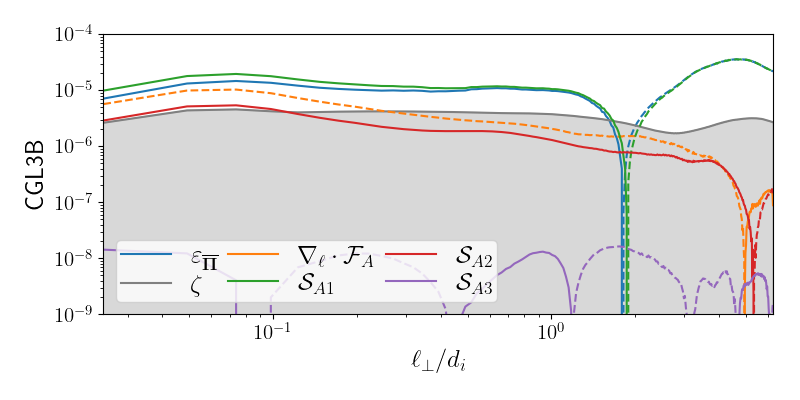
\includegraphics[width=1\linewidth,trim=0cm 1cm 0cm 1cm, clip=true]{./Part_3/images_ch3/CGL3B_compa_cgl}
 % % \includegraphics[width=1\linewidth,trim=0cm 1cm 0cm 1cm, clip=true]{./Part_3/images_ch3/CGL3_compa_cgl}
% \cprotect\caption{Représentation \acs{1D} en fonction de $\ell_{\perp}$ du détail de $\varepsilon_{\overline{\boldsymbol{\Pi}}}$ (bleu). Orange : $\nabla_{\boldsymbol{\ell}} \cdot \boldsymbol{\mathcal{F}_A}$. Vert : $\mathcal{S}_{A1}$. Rouge : $\mathcal{S}_{A2}$. Violet : $\mathcal{S}_{A3}$. Gris : niveau d'erreur $\zeta$. Les termes présents dans la zone grise délimitée par $\zeta$ sont supposés négligeables. Simu : CGL3B. }
% \label{fig:detail_simu_CGL3B}
% \end{figure}

\subsection{Une gamme d'échelle intermédiaire : CGL5}
\begin{figure}[!ht]
 \centering
 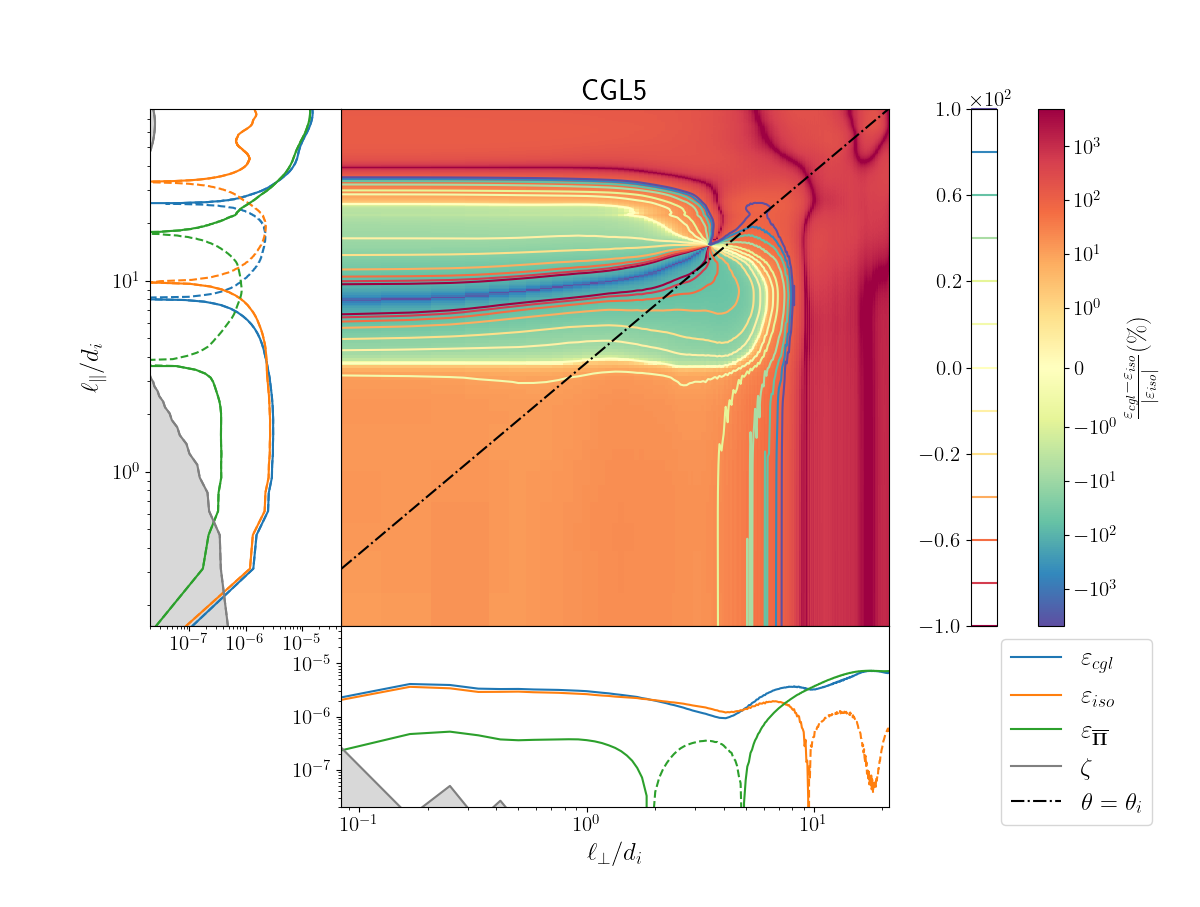
\includegraphics[width=0.95\linewidth,trim=1cm 1cm 0cm 2cm, clip=true]{./Mainmatter/Part_3/images_ch3/CGL5_panel_isocgl_percent}
 \cprotect\caption{Simu : CGL5. Représentation \sacro{2D} en fonction de \ensuremath{\ell_{\perp}} et \ensuremath{\ell_{\parallel}} de \ensuremath{\varepsilon_{cgl}-\varepsilon_{iso}} par rapport à \ensuremath{|\varepsilon_{iso}|} en \ensuremath{\%}, entourée des représentations \cacro{1D} en fonction de \ensuremath{\ell_{\perp}} (bas) et \ensuremath{\ell_{\parallel}} (gauche) de \ensuremath{\varepsilon_{iso}} (orange), \ensuremath{\varepsilon_{cgl}} (bleu), \ensuremath{\varepsilon_{\overline{\boldsymbol{\Pi}}}} (vert) et \ensuremath{\zeta} (gris). }
\label{fig:trip_CGL5}
\end{figure}

 La gamme d'échelles accessible via CGL5 est située entre celles de CGL2 et celles de CGL3 afin de couvrir la transition entre la zone \cacro{MHD} et la zone \cacro{Hall}, tout en gardant éloignées les échelles impactées par l'injection d'énergie. %Sur la \tabref{tab:stat_CGL}, on voit que sa compression est similaire à celle de CGL2, les termes purement compressibles seront encore une fois négligeables.
 L'écart-type de sa distribution est aussi de l'ordre de celui de CGL2, tout comme son étalement dans le diagramme de la \figref{fig:diag_simu_CGL}, mais sa position centrale y est plus proche de celle de CGL3. Le comportement observé pourrait donc être en faveur de la conjecture d'un impact de la moyenne de $a_{pi}$ ou de celle d'un impact des fluctuations sur la contribution du taux de cascade dépendant de l'anisotropie de pression. 
 
 % \begin{figure}[!ht]
 %  \centering
 %  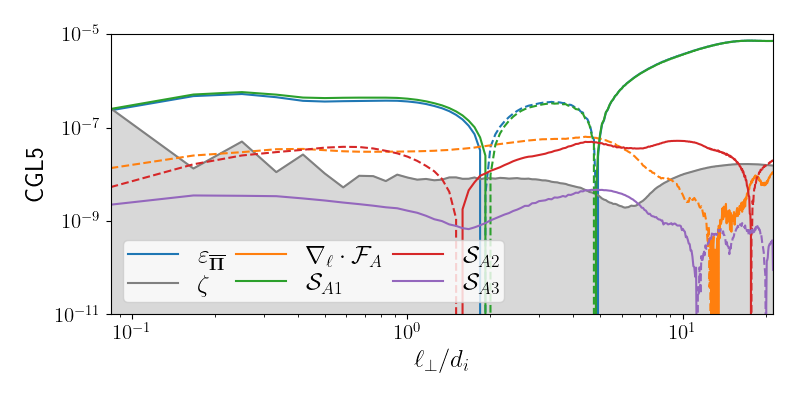
\includegraphics[width=1\linewidth,trim=0cm 1cm 0cm 1cm, clip=true]{./Part_3/images_ch3/CGL5_compa_cgl}
 % \cprotect\caption{Simu : CGL5. Représentation 1D en fonction de $\ell_{\perp}$ du détail de $\varepsilon_{\overline{\boldsymbol{\Pi}}}$ (bleu). Orange : $\nabla_{\boldsymbol{\ell}} \cdot \boldsymbol{\mathcal{F}_A}$. Vert : $\mathcal{S}_{A1}$. Rouge : $\mathcal{S}_{A2}$. Violet : $\mathcal{S}_{A3}$. Gris : niveau d'erreur $\zeta$. Les termes présents dans la zone grise délimitée par $\zeta$ sont supposés négligeables. }
 % \label{fig:detail_simu_CGL5}
 % \end{figure}
 
 Sur le triptyque obtenu pour CGL5 (\figref{fig:trip_CGL5}), on observe un comportement similaire à celui de CGL3. Dans la zone inertielle ($\ell_{\perp} \in [\num{0.3};\num{5}]$\footnote{La taille de la zone inertielle perpendiculaire dans la représentation \cacro{1D} de la \figref{fig:trip_CGL5} est réduite à cause de la \og bulle \fg{} négative parallèle et du filtrage angulaire. La valeur maximale est donc estimée à partir de la représentation \sacro{2D}.}), la contribution de $\varepsilon_{\overline{\boldsymbol{\Pi}}}$ est de l'ordre de $\SI{10}{\%}$ de $\varepsilon_{iso}$. Ces résultats confirment que le comportement de CGL3 n'est pas un cas particulier et se placent en faveur de la moyenne de $a_{pi}$ plutôt que de ses fluctuations. De plus, l'augmentation à grande échelle visible pour CGL3 s'est déportée avec le forçage, confirmant qu'elle est intrinsèque à la zone d'injection de l'énergie dans la cascade.  


\subsection{Une initialisation anisotrope $a_{piI} = 4$ : CGL6}
\begin{figure}[!ht]
 \centering
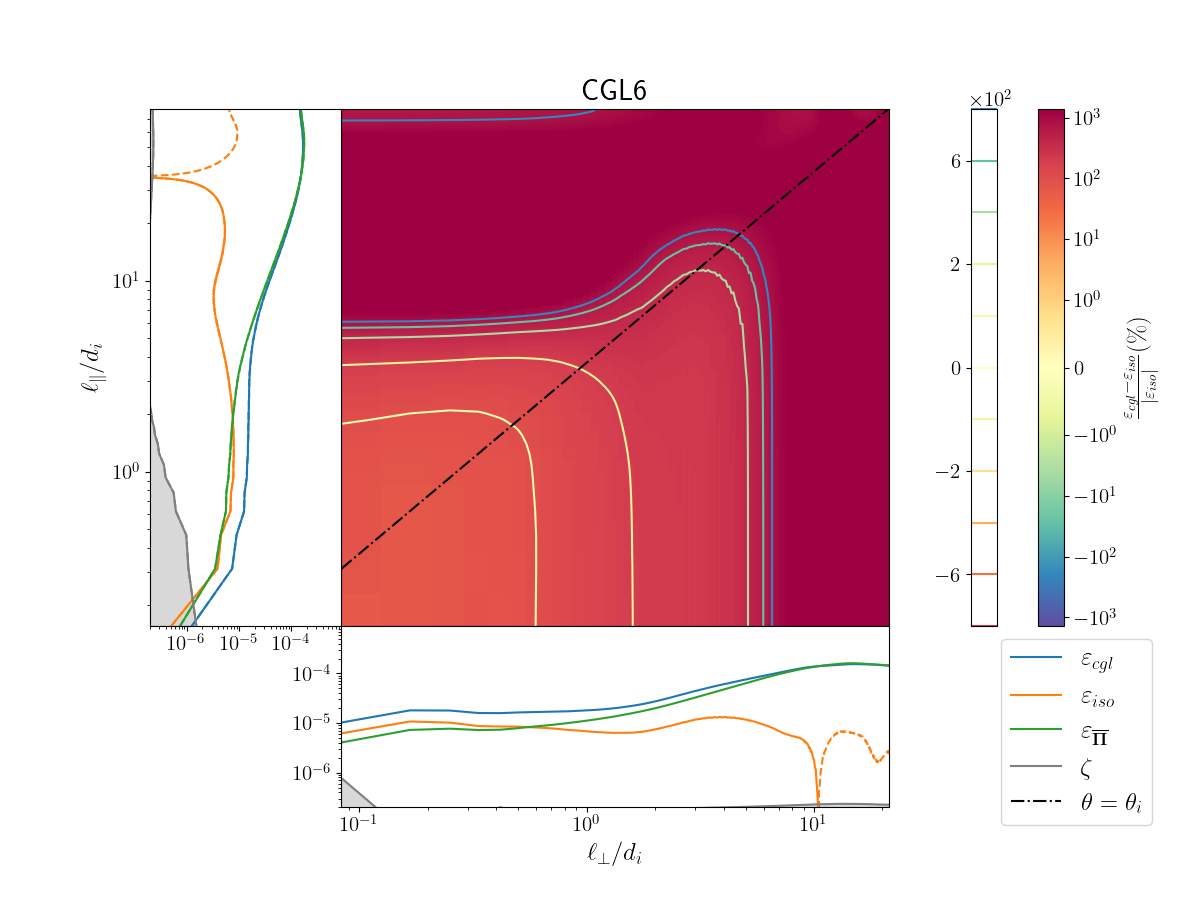
\includegraphics[width=0.95\linewidth,trim=1cm 1cm 0cm 2cm, clip=true]{./Mainmatter/Part_3/images_ch3/CGL6_panel_isocgl_percent}
\cprotect\caption{Simu : CGL6. Représentation \sacro{2D} en fonction de \ensuremath{\ell_{\perp}} et \ensuremath{\ell_{\parallel}} de \ensuremath{\varepsilon_{cgl}-\varepsilon_{iso}} par rapport à \ensuremath{|\varepsilon_{iso}|} en \ensuremath{\%}, entourée des représentations \cacro{1D} en fonction de \ensuremath{\ell_{\perp}} (bas) et \ensuremath{\ell_{\parallel}} (gauche) de \ensuremath{\varepsilon_{iso}} (orange), \ensuremath{\varepsilon_{cgl}} (bleu), \ensuremath{\varepsilon_{\overline{\boldsymbol{\Pi}}}} (vert) et \ensuremath{\zeta} (gris). }
\label{fig:trip_CGL6}
\end{figure}
La dernière simulation lancée est CGL6. Elle est basée sur CGL5 mais initialisée avec une pression anisotrope : $a_{piI} = 4 $. Le but de cette simulation est double :
\begin{itemize}
    \item vérifier si l'un des comportements observés précédemment pour notre correction se maintient lorsque la simulation est initialisée anisotropiquement,
    \item se rapprocher du critère miroir.
\end{itemize}
Des valeurs de $a_{piI}$ plus importantes ont été testées, mais seule la simulation avec $a_{piI} = 4 $ a pu être numériquement stabilisée. 

 Comme on peut le voir sur la \tabref{tab:stat_CGL} et sur la \figref{fig:diag_simu_CGL} (violet), cette simulation se maintient au niveau de $a_{piI}$. En fait, c'est la seule simulation montrant un $a_{pi0}$ aussi proche de sa condition initiale, l'écart n'étant que de $\SI{3}{\%}$. Pour ce qui est du but de se rapprocher du critère miroir, le diagramme nous indique que quelques points de CGL6 sont situés au-dessus du critère miroir. Le développement d'instabilité miroir semble donc permis dans cette simulation. 
 
 Sur la \figref{fig:trip_CGL6},  $\varepsilon_{\overline{\boldsymbol{\Pi}}}$ est entièrement positif. Son niveau est de l'ordre de $\SI{70}{\%}$ de $\varepsilon_{iso}$ aux échelles inertielles, c'est-à-dire pour $\ell_{\perp} \in [\num{0.3};\num{1}]$. Il a donc bien augmenté par comparaison avec les $\SI{10}{\%}$ et $\SI{30}{\%}$ précédents. Par comparaison avec CGL5, la gamme d'échelles inertielles est réduite par l'augmentation de $\varepsilon_{\overline{\boldsymbol{\Pi}}}$ qui est plus étalée. %Les termes purement compressibles sont toujours de l'ordre de l'erreur numérique.


% \begin{figure}[!ht]
%  \centering
% 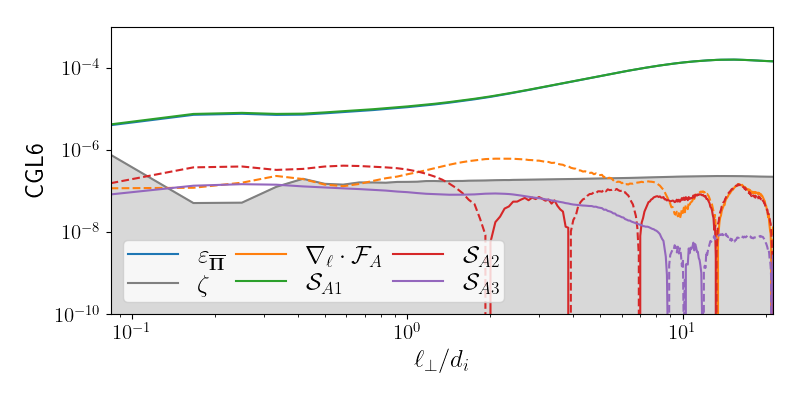
\includegraphics[width=1\linewidth,trim=0cm 1cm 0cm 1cm, clip=true]{./Part_3/images_ch3/CGL6_compa_cgl}
% \cprotect\caption{Simu : CGL6. Représentation 1D en fonction de $\ell_{\perp}$ du détail de $\varepsilon_{\overline{\boldsymbol{\Pi}}}$ (bleu). Orange : $\nabla_{\boldsymbol{\ell}} \cdot \boldsymbol{\mathcal{F}_A}$. Vert : $\mathcal{S}_{A1}$. Rouge : $\mathcal{S}_{A2}$. Violet : $\mathcal{S}_{A3}$. Gris : niveau d'erreur $\zeta$. Les termes présents dans la zone grise délimitée par $\zeta$ sont supposés négligeables. De haut en bas : CGL3, CGL5 et CGL6. }
% \label{fig:detail_simu_CGL6}
% \end{figure}

\section{Synthèse de l'étude préliminaire des simulations CGL-MHD-Hall-\ensuremath{\nabla P_e}}
\label{synth-33}

{\bf Les résultats présentés dans ce chapitre nous permettent de valider numériquement l'apport de la correction dépendant de l'anisotropie de pression dans le cas quasi-incompressible. Ils nous confirment aussi que, dans un cadre quasi-incompressible, le terme dominant est celui qui vient former la correction de \cacro{PP98} dans la limite incompressible gyrotrope (Chapitre \ref{ch-22}).} Cela implique que la première correction devant être appliquée dans un plasma quasi-incompressible tel que le vent solaire n'est peut-être pas la compression mais plutôt l'anisotropie de pression. Cette étude numérique n'est cependant qu'à un stade préliminaire. En effet, nous n'avons pas encore convergé sur l'interprétation d'un certain nombre d'éléments et, comme nous venons de le voir, elle soulève un nombre important de questions.


\begin{figure}[!ht]
 \centering
 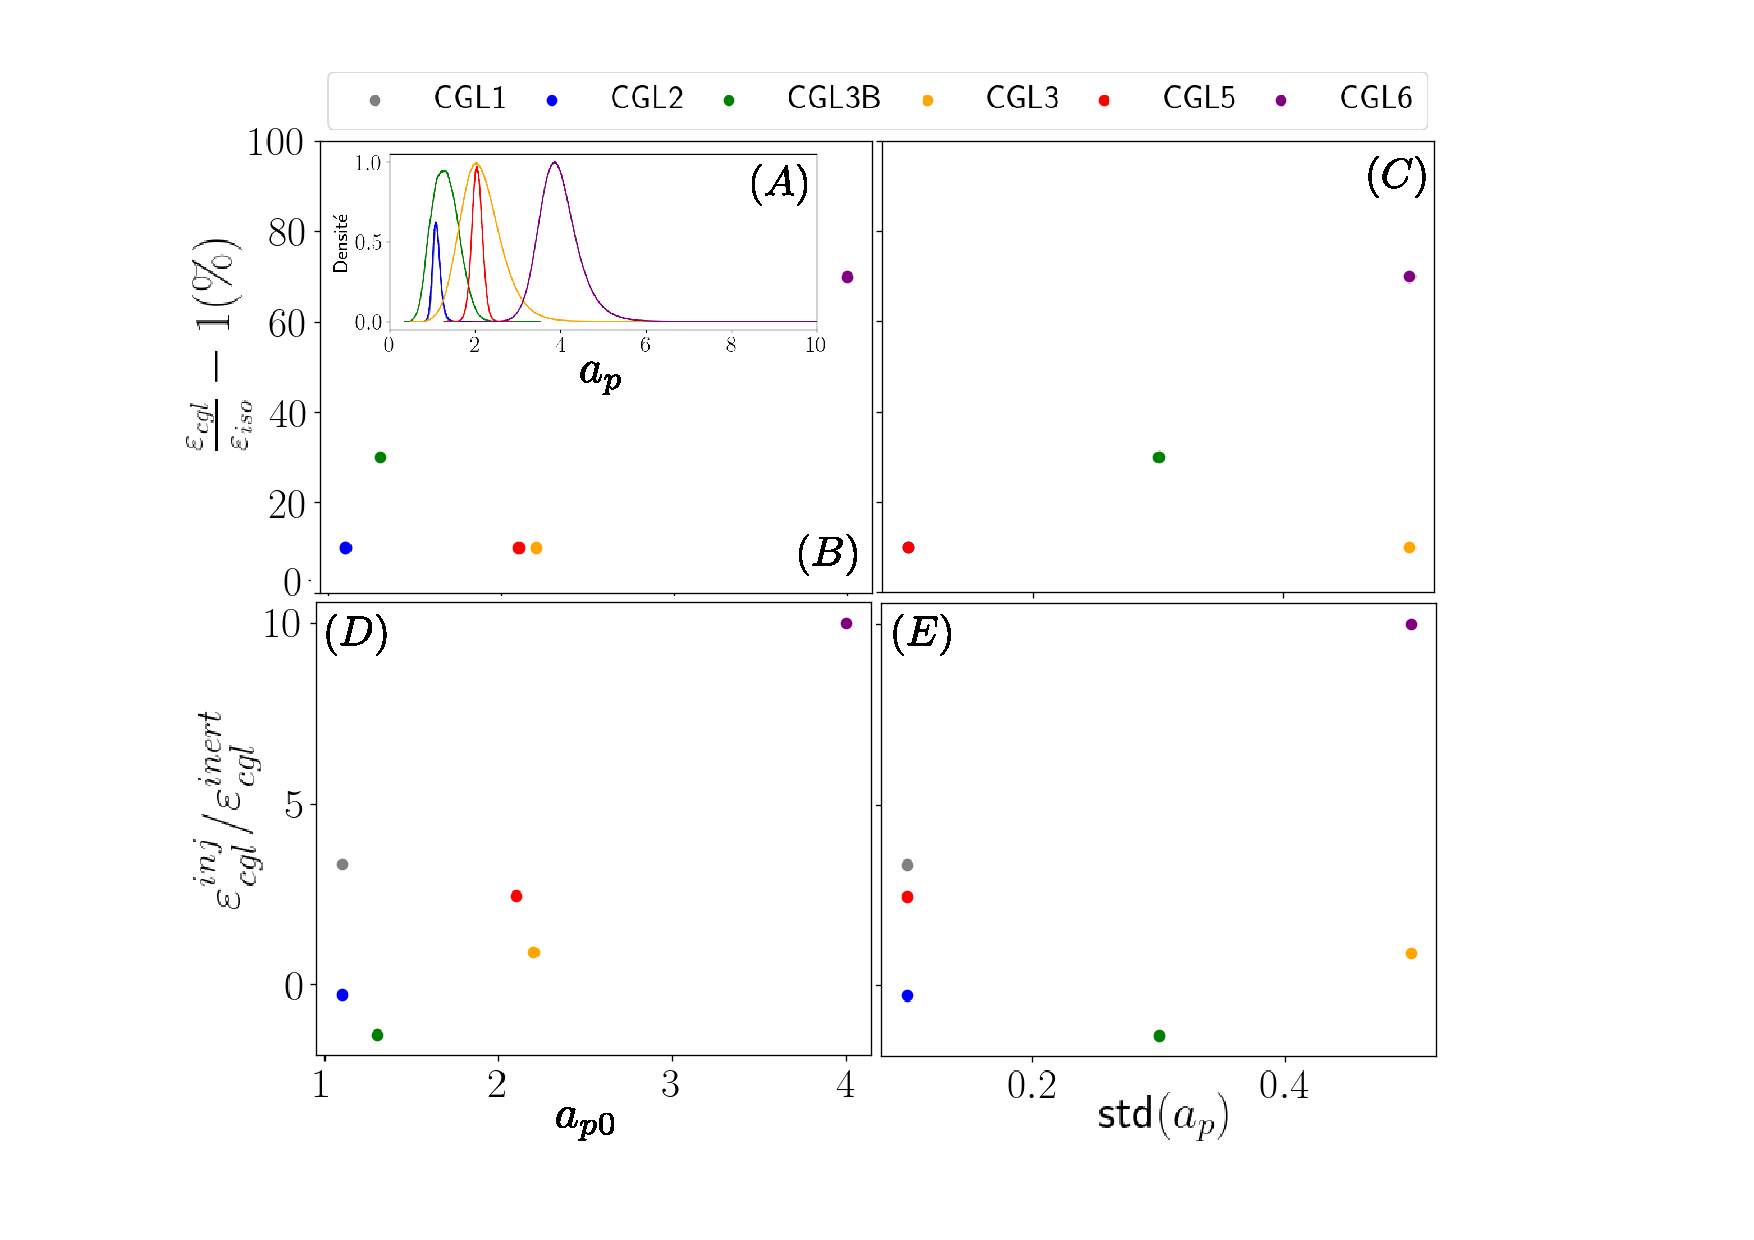
\includegraphics[width=0.9\linewidth,trim=3cm 1cm 5cm 1cm, clip=true]{./Mainmatter/Part_3/images_ch3/scattersimu}
\cprotect\caption{Résumé de l'étude préliminaire sur l'effet de l'anisotropie de pression sur le taux de transfert non linéaire en fonction de \ensuremath{a_{pi0}} (première colonne) et de \ensuremath{\text{std}(a_p)} (deuxième colonne). Chaque simulation est associée à une couleur (même association que pour la \figref{fig:diag_simu_CGL}). (A) : histogramme de \ensuremath{a_p}, CGL1 y est confondu avec CGL2. (B) et (C) : apport de la contribution de la pression anisotrope. (D) et (E) : impact de l'augmentation dans la zone de forçage de la contribution anisotrope sur le niveau du taux de transfert total mesuré dans la zone inertielle.}
\label{fig:scattersimu}
\end{figure}
 
 On propose une synthèse à travers la \figref{fig:scattersimu}. Sur le graphique $(A)$ sont repris les histogrammes de $a_{pi}$, (CGL1 y est confondu avec CGL2). Les simulations sont ordonnées par couleur et comportement : les simulations présentant un changement de signe sont en gris (CGL1), bleu (CGL2) et vert (CGL3B). Celles  montrant un signe quasiment isotrope à l'exception d'une \og bulle \fg{} dans la direction parallèle sont en jaune (CGL3) et rouge (CGL5). La dernière simulation, initialisée avec $a_{piI}  = 4$, montrant une contribution anisotrope entièrement positive, est donnée en violet (CGL6). Deux paramètres liés à la distribution de $a_{pi}$ ont été abordés : la moyenne $a_{pi0}$ (graphique $(B)$ et $(C)$) et l'écart-type $\text{std}(a_{pi})$ (graphique $(D)$ et $(E)$). En fonction de $a_{pi0}$, les simulations se comportant similairement restent groupées, contrairement à $\text{std}(a_{pi})$. $a_{pi0}$ semble donc être un meilleur paramètre que $\text{std}(a_{pi})$. Sur le graphique $(B)$, sont placées les estimations de la contribution anisotrope au taux de cascade dans la zone inertielle. On y observe que CGL3B et CGL6 s'écartent du résultat des autres simulations. Ce résultat est inattendu pour CGL3B (ou CGL3 et CGL5). Si $a_{pi0}$ est bien le paramètre important dans l'impact des anisotropies de pression sur la cascade et que CGL3B est bien valable et n'est pas une exception, alors il pourrait exister un processus qui viendrait inverser, pour quelques $a_{pi0}$, la tendance croissante de la contribution anisotrope dans la zone inertielle. Pour ce qui est du rapport entre le taux de transfert non linéaire estimé dans la zone de forçage et le taux de cascade inertielle (graphique (D)), il semble globalement croitre en fonction de $a_{pi0}$. Il serait intéressant d'y évaluer plus précisément l'impact de l'injection d'énergie afin de vérifier si un autre processus intervient. 
 
 Ces graphiques, contenant un nombre limité de points lié au nombre de simulations à disposition, ne sont, bien évidemment, que des outils de spéculation, synthétisant cette étude préliminaire et permettant de dégager des tendances pour lesquelles l'analyse pourra être approfondie.




% \section{Etude de spectre } \label{sec-334}

% Sachant que le forçage se fait avec des modes aléatoires de fréquences proches de celle du mode d'Alfvén et que des études telles celle de \cite{brodiano_spatiotemporal_2021} ont relié le choix de forçage aux ondes dominant la simulation, observer une cascade développée par des ondes d'Alfvén dans nos simulations serait tout à fait réaliste. Si l'on regarde les spectres de champs magnétiques parallèle et perpendiculaire de CGL2 par exemple (\figref{fig:spectre}), on remarque que le spectre d'énergie magnétique est dominé par les fluctuations perpendiculaires au champ magnétique ambiant et on y retrouve les pentes turbulentes en $-5/3$ (zone MHD) et en $-7/3$ (zone Hall).  Un tel résultat est une signature de la nature alfvénique de la cascade turbulente. Il n'est donc pas impossible que la correction d'anisotropie de pression soit dominé par la correction firehose. 
% \begin{figure}[!ht]
%  \centering
% 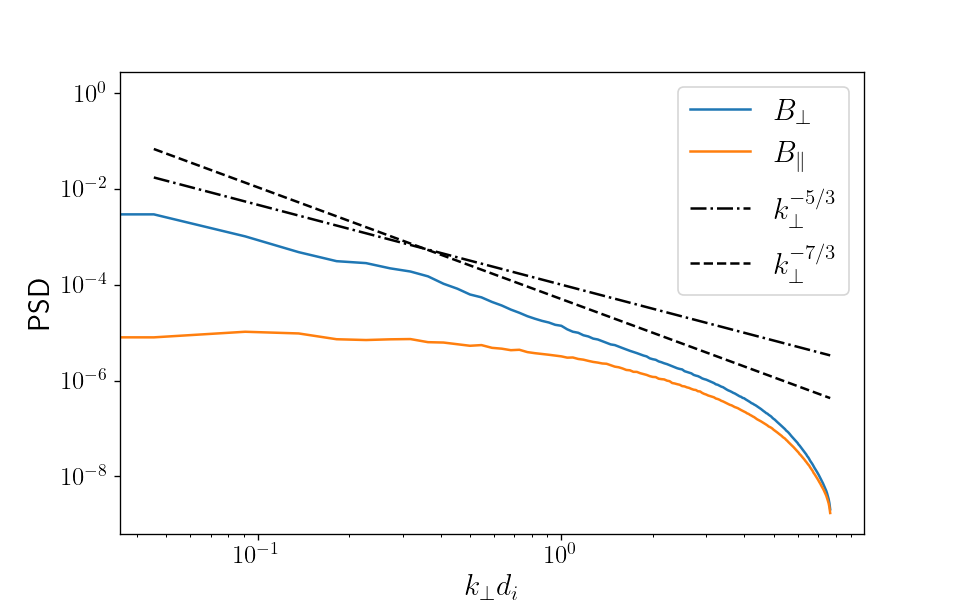
\includegraphics[width=0.95\linewidth,trim=0cm 0cm 0cm 0cm, clip=true]{./Part_3/images_ch3/CGL2_spectre}
% \cprotect\caption{Simu : CGL2. Spectre d'énergie magnétique perpendiculaire et parallèle en fonction de $k_{\perp}d_i$}
% \label{fig:spectre}
% \end{figure}

% Sur le spectre des fluctuations perpendiculaires, on peut remarquer une bosse en $k_{\perp}d_i = 0.3$, cela correspondrait à $\ell_{\perp}/d_i = 21 $. Si l'on regarde sur le triptyque associé à CGL2 (\figref{fig:trip_CGL1-2}), on remarque que cette échelle correspond au début de l'augmentation de $\varepsilon_{\overline{\boldsymbol{\Pi}}}$. 

% Les spectres de CGL5 et CGL6 sont plus complexes à analyser, la contribution des fluctuations parallèles au spectre total prend de l'importance dans la zone Hall, comme on peut le voir pour sur la \figref{fig:spectre_CGL6}. Serait la signature d'une cascade d'ondes magnétosonores ?
% \begin{figure}[!ht]
%  \centering
% 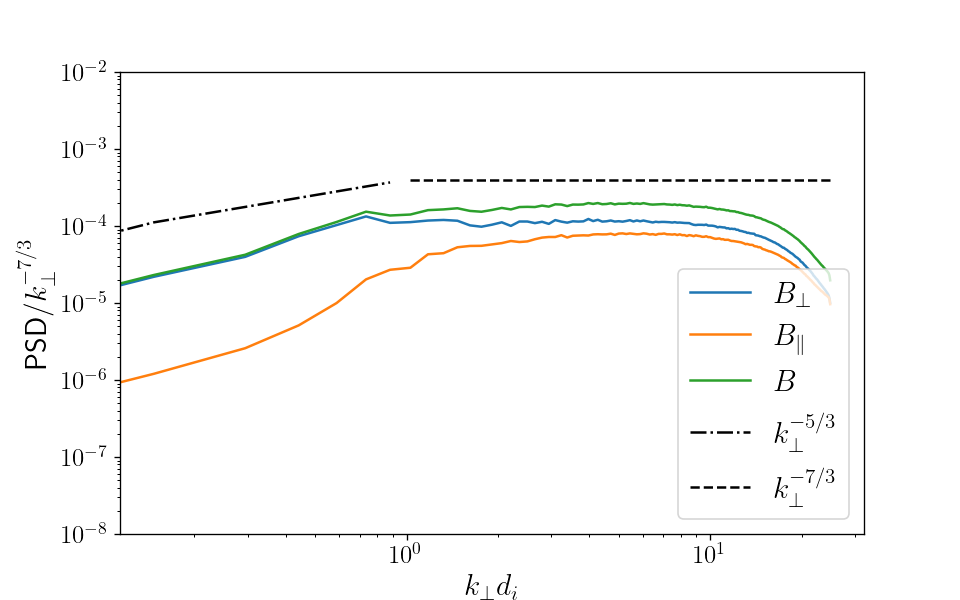
\includegraphics[width=0.95\linewidth,trim=0cm 0cm 0cm 0cm, clip=true]{./Part_3/images_ch3/CGL6_spectre}
% \cprotect\caption{Simu : CGL6. Spectre d'énergie magnétique perpendiculaire et parallèle en fonction de $k_{\perp}d_i$. Le spectre est compensé par la pente $-7/3$ attendue dans la zone inertielle Hall.}
% \label{fig:spectre_CGL6}
% \end{figure}
